\documentclass{article}       % use "amsart" instead of "article" for AMSLaTeX format
\usepackage{geometry}                              % See geometry.pdf to learn the layout options. There are lots.
%\geo4metry{landscape}                            % Activate for for rotated page geometry
%\usepackage[parfill]{parskip}                  % Activate to begin paragraphs with an empty line rather than an indent
\usepackage{graphicx}                         % Use pdf, png, jpg, or eps§ with pdflatex; use eps in DVI mode
% TeX will automatically convert eps --> pdf in pdflatex         
\usepackage{amssymb}
\usepackage{amsmath}
\usepackage{mathtools}
\usepackage{booktabs}
\usepackage{tabto}
\usepackage{algorithm}
\usepackage{algpseudocode}
\usepackage{tikz}

\DeclarePairedDelimiter\ceil{\lceil}{\rceil}
\DeclarePairedDelimiter\floor{\lfloor}{\rfloor}


\usetikzlibrary{shapes.geometric}
\tikzset{
        buffer/.style={
                draw,
                shape border rotate=0,
                regular polygon,
                regular polygon sides=3,
                fill=white,
                node distance=2cm,
                minimum height=4em
        }
}
\tikzset{
        buffer2/.style={
                draw,
                shape border rotate=180,
                regular polygon,
                regular polygon sides=3,
                fill=white,
                node distance=2cm,
                minimum height=4em
        }
}



\title{Adv Data Struct $\&$ Algorithm: Homework 4}
\author{Zimian Li}

\begin{document}
        
\maketitle
\begin{enumerate}
	\item[1.] Consider a universe $\mathcal{U}$ of keys each of which is $b$ bits long. You want to construct a hash table of size $m=2^a$. To select your hash function $h$, you build a random binary matrix $M$ and let $h_M(x)=M\times x$, with the caveat that addition is done modulo 2. Your set $\mathcal{H}$ of hash functions is the set of all possible binary matrices.
	\begin{enumerate}
		\item[(a)] What should be the dimensions of matrix $M$?\newline\newline
		We can write the hash function as $h_M(x)=M\times (x_1,x_2, ..., x_b) = (y_1, y_2, ..., y_a)$. Obviously, matrix $M$ should be $b\times a$.\newline
		\item[(b)] How big is $\mathcal{H}$?\newline\newline
		Because the size of $M$ is $ba$, and every element of it could be 0 or 1, therefore, the total number of all kinds of $M$ is $2^{ba}$. It's also the size of $\mathcal{H}$.\newline
		\item[(c)] Show that $\mathcal{H}$ is universal.\newline\newline
		\textbf{Proof:} Suppose $k, l$ be two arbitrary distinct keys from $\mathcal{U}$, and $k = (k_1, k_2, ..., k_b)$ and $l = (l_1, l_2, ..., l_b)$. And Pick a random hash function $h_M(x)=M\times x$ from $\mathcal{H}$.\newline
		Therefore, $h(k) = ((\sum_{i=1}^{b} k_iM_{i1}) \mod 2, (\sum_{i=1}^{b} k_iM_{i2}) \mod 2, ..., (\sum_{i=1}^{b} k_iM_{ia}) \mod 2)$, and $h(l) = ((\sum_{i=1}^{b} l_iM_{i1}) \mod 2, (\sum_{i=1}^{b} l_iM_{i2}) \mod 2, ..., (\sum_{i=1}^{b} l_iM_{ia}) \mod 2)$. If $h(k)=h(l)$, then for an arbitrary $j$(j is in range 1 to a), $(\sum_{i=1}^{b} k_iM_{ij}) \mod 2 = (\sum_{i=1}^{b} l_iM_{ij}) \mod 2$. That means $(\sum_{i=1}^{b} k_iM_{ij})$ and  $(\sum_{i=1}^{b} l_iM_{ij})$ have the same parity.\newline
		\textbf{Claim:} Pr($(\sum_{i=1}^{b} k_iM_{ij})$ is even) = Pr($(\sum_{i=1}^{b} k_iM_{ij})$ is odd) = 1/2.\newline
		Proof: $k_i$ and $M_{ij}$ are all 0 or 1, so there are 4 cases (with equal possibility) of $k_iM_{ij}$:\newline
		1) $0\cdot 0 = 0$\newline
		2) $0\cdot 1 = 0$\newline
		3) $1\cdot 0 = 0$\newline
		4) $1\cdot 1 = 1$\newline
		Obviously, the parity of $(\sum_{i=1}^{b} k_iM_{ij})$ only depends on the number of $1\cdot 1$. And the chance is equal for the number of $1\cdot 1$ is even or odd. Therefore, Pr($(\sum_{i=1}^{b} k_iM_{ij})$ is even) = Pr($(\sum_{i=1}^{b} k_iM_{ij})$ is odd) = 1/2. It's also same for $(\sum_{i=1}^{b} l_iM_{ij})$.\newline
		Hence, Pr($(\sum_{i=1}^{b} k_iM_{ij})$ and  $(\sum_{i=1}^{b} l_iM_{ij})$ have the same parity) = Pr($(\sum_{i=1}^{b} k_iM_{ij})$ is even and  $(\sum_{i=1}^{b} l_iM_{ij})$ is even) + Pr($(\sum_{i=1}^{b} k_iM_{ij})$ is odd and  $(\sum_{i=1}^{b} l_iM_{ij})$ is odd) = $1/2 \cdot 1/2 + 1/2 \cdot 1/2 = 1/2$.\newline
		Therefore, Pr($h(k) = h(l)$) = Pr($(\sum_{i=1}^{b} k_iM_{i1})$ and  $(\sum_{i=1}^{b} l_iM_{i1})$ have the same parity) $\cdot$ Pr($(\sum_{i=1}^{b} k_iM_{i2})$ and  $(\sum_{i=1}^{b} l_iM_{i2})$ have the same parity) $\cdot$ ... $\cdot$ Pr($(\sum_{i=1}^{b} k_iM_{ia})$ and  $(\sum_{i=1}^{b} l_iM_{ia})$ have the same parity) = $(\frac{1}{2})^a$ = $(\frac{1}{2^a})$ = $\frac{1}{m}$. So finally, I can conclude $\mathcal{H}$ is universal.\newline
	\end{enumerate}
	\item[2.] Hashing a set of $n$ keys into a table of size $m$ requires $\Omega (n+m)$ time due to the fact that the table needs to be initialized. This is inefficient when $n=o(m)$. Describe a method that avoids initializing the hash table, possibly at the expense of some additional memory.\newline\newline
	If not initializing the hash table, we need another container to save these messages.\newline 
	1) If choosing a linear container such as an array, every time hashing a new key, I need to check this array if this key already exists, if so just update this key, if not add this key to the array. Thus, the time cost of hashing $n$ keys is $O(n^2)$, I can choose it if $n^2 < n+m$.\newline
	2) I can also choose to maintain a binary search tree for keys, then the time cost of hashing $n$ keys is $O(n\log n)$, it's better than the linear container, I can choose it if $n\log n < n+m$.\newline
	\item[3.] Using comparison trees, prove lower bounds for the following problems. In each case, make sure to clearly indicate the number of leaves in the tree from which you compute the lower bound.
	\begin{enumerate}
		\item[(a)] Given two sorted lists $A$ and $B$ of size $n$ each, merge them into a single sorted list $C$.\newline\newline
		\begin{figure}[H]
			\centering
			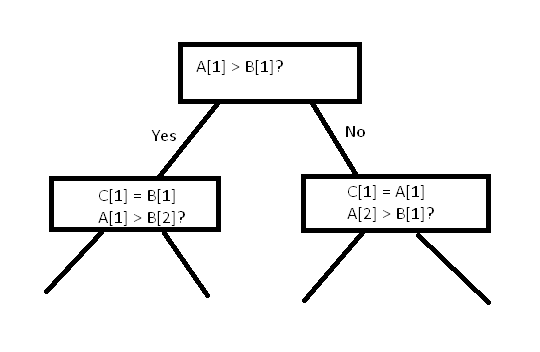
\includegraphics[width=10cm]{ct1}
			\caption{(ct1)}
			\label{ct1}
		\end{figure}
		The image above is the initial part of the comparison tree, obviously, the number of leaves is the number of permutations of $C$. For the size of $A$ and $B$ are both $n$, the number of permutations of $C$ should be $2n \choose n$. Therefore, the height of this comparison tree is $\log (2\cdot {2n \choose n} -1)$.\newline
		${2n \choose n} = \frac{2n!}{(n!)^2} = \frac{(2n)\cdot (2n-1) \cdot ... \cdot (n+1)}{n\cdot (n-1) \cdot ... \cdot 1} = \frac{2n}{n} \cdot \frac{2n-1}{n-1} \cdot ... \cdot \frac{n+1}{1} > (\frac{2n}{n})^n = 2^n$.\newline
		Therefore, $\log (2\cdot {2n \choose n} -1) \in \Omega (n)$. It's the lower bound of this problem.\newline
		\item[(b)] Given an array $A[1:n]$ of values from a totally ordered set, rearrange $A$ so that the $n/2$ smallest values appear on the left and the $n/2$ largest appear on the right.\newline\newline
		Consider the comparison tree, the leaves are all permutations that meeting the $n/2$ smallest values appear on the left and the $n/2$ largest appear on the right. The number is $(n/2)!^2$. So the height of the comparison tree is $\log (2\cdot (n/2)!^2 - 1) \in \Omega(n\log n)$. Hence, the lower bound is $\Omega(n\log n)$.
	\end{enumerate}
	\item[4.] Consider a min-max heap $H$ with $n$ elements. $H$ can be viewed a complete binary tree that uses the same array representation used in ordinary heaps.
	\begin{enumerate}
		\item[(a)] INSERT$(H,n,x)$ inserts an element with key $x$ into $H$. Describe how to implement INSERT in $O(\log \sqrt{n})$ time.\newline\newline
		It's similar with the insertion of the ordinary heap, the difference is that we need to compare the new key with the parent of the parent of itself (grandparent!). And we need to calculate its depth ($\floor{\log (i+1)}$) to decide it's in min-level or max-level. The time cost is $O(\frac{1}{2}\log n) = O(\log \sqrt{n})$.
		 \begin{algorithm}[H]
			\caption{INSERT}
			\small
			\begin{algorithmic}[1]
				\Procedure {INSERT}{H, n, x}
				\State increase H with a new slot, n += 1
				\State H[n-1] = x, i = n-1
				\If {$\floor{\log (i+1)}$ is even}
				\While {i $\geq$ 0 and H[Parent(Parent(i))] $>$ H[i]}
				\State exchange   H[Parent(Parent(i))], H[i]
				\State i $\gets$ Parent(Parent(i))
				\EndWhile
				\Else
				\While {i $\geq$ 1 and H[Parent(Parent(i))] $<$ H[i]}
				\State exchange   H[Parent(Parent(i))], H[i]
				\State i $\gets$ Parent(Parent(i))
				\EndWhile
				\EndIf
				\EndProcedure
			\end{algorithmic}\label{p1}
		\end{algorithm}	
		\item[(b)] DELETEMIN$(H,n)$ deletes and returns the element with minimum key from $H$. Describe an efficient implementation of DELETEMIN and analyze its running time.\newline\newline
		It's also similar with the ordinary heap. The DELETEMIN operation is based on MIN-HEAPIFY, the differences is that we need to consider its all 4 grandchildren, the time cost is also $O(\log \sqrt{n})$ for only need to consider min-level.
		\begin{algorithm}[H]
			\caption{MIN-HEAPIFY}
			\small
			\begin{algorithmic}[1]
				\Procedure {MIN-HEAPIFY}{H,  n, i}
				\State ll $\gets$ LEFT(LEFT(i))
				\State lr $\gets$ LEFT(RIGHT(i))
				\State rl $\gets$ RIGHT(LEFT(i))
				\State rr $\gets$ RIGHT(RIGHT(i))
				\If {ll $<$ n and H[ll] $<$ H[i]}
				\State smallest = ll
				\Else \State smallest = i
				\EndIf
				\If {lr $<$ n and H[lr] $<$ H[smallest]}
				\State smallest = lr
				\EndIf
				\If {rl $<$ n and H[rl] $<$ H[smallest]}
				\State smallest = rl
				\EndIf
				\If {rr $<$ n and H[rr] $<$ H[smallest]}
				\State smallest = rr
				\EndIf
				\If {smallest != i}
				\State exchange H[smallest], H[i]
				\State MIN-HEAPIFY(H, n, smallest)
				\EndIf				
				\EndProcedure
			\end{algorithmic}\label{p1}
		\end{algorithm}	
		\begin{algorithm}[H]
			\caption{DELETEMIN}
			\small
			\begin{algorithmic}[1]
				\Procedure {DELETEMIN}{H,  n}
				\State min $\gets$ H[0]	
				\State H[0] $\gets$ H[n-1]
				\State n -= 1
				\State MIN-HEAPIFY(H, n, 0)	
				\State \Return min	
				\EndProcedure
			\end{algorithmic}\label{p1}
		\end{algorithm}	
		\item[(c)] DELETEMAX$(H,n)$ deletes and returns the element with maximum key from $H$. Describe an efficient implmentation of DELETEMAX and analyze its running time.\newline\newline
		It's similar with DELETEMIN, based on MAX-HEAPIFY. Another point is that the second level has 2 max nodes, we need to compare them to decide which one is the true max. The time complexity is $O(\log \sqrt{n})$.
		\begin{algorithm}[H]
			\caption{MAX-HEAPIFY}
			\small
			\begin{algorithmic}[1]
				\Procedure {MAX-HEAPIFY}{H,  n, i}
				\State ll $\gets$ LEFT(LEFT(i))
				\State lr $\gets$ LEFT(RIGHT(i))
				\State rl $\gets$ RIGHT(LEFT(i))
				\State rr $\gets$ RIGHT(RIGHT(i))
				\If {ll $<$ n and H[ll] $>$ H[i]}
				\State largest = ll
				\Else \State largest = i
				\EndIf
				\If {lr $<$ n and H[lr] $>$ H[largest]}
				\State largest = lr
				\EndIf
				\If {rl $<$ n and H[rl] $>$ H[largest]}
				\State largest = rl
				\EndIf
				\If {rr $<$ n and H[rr] $>$ H[largest]}
				\State largest = rr
				\EndIf
				\If {largest != i}
				\State exchange H[largest], H[i]
				\State MAX-HEAPIFY(H, n, largest)
				\EndIf				
				\EndProcedure
			\end{algorithmic}\label{p1}
		\end{algorithm}	
		\begin{algorithm}[H]
			\caption{DELETEMAX}
			\small
			\begin{algorithmic}[1]
				\Procedure {DELETEMAX}{H,  n}
				\If {H[1] $>$ H[2]}
				\State max = H[1]
				\State max-index = 1
				\Else
				\State max = H[2]
				\State max-index = 2
				\EndIf 
				\State H[max-index] $\gets$ H[n-1]
				\State n -= 1
				\State MAX-HEAPIFY(H, n, max-index)	
				\State \Return max	
				\EndProcedure
			\end{algorithmic}\label{p1}
		\end{algorithm}	
		\item[(d)] Given an array $A[1:n]$ of integers, with no particular structure, can you rearrange $A$ into a min-max heap on $o(n\log n)$ time? Explain.\newline\newline
		All I can do is like below. Its time complexity is $2 \cdot \frac{n}{4} \cdot O(\log \sqrt{n}) = O(\frac{n}{4}\log n) = O(n\log n)$. Consider a comparison tree, to build a min-max heap is based on comparison. The number of leaves is $n!$, thus the height is at least $\Omega(\log n!) \approx \Omega(n\log n)$. The lower bound is $\Omega(n\log n)$, not possible to find a $o(n\log n)$ alorithm.
		\begin{algorithm}[H]
			\caption{BUILD-MIN-MAX-HEAP}
			\small
			\begin{algorithmic}[1]
				\Procedure {BUILD-MIN-MAX-HEAP}{A}
				\For {i $\gets$ $\floor{length(A)/2}$} downto 1
				\If {$\floor{\log (i)}$ is even}
				\State MIN-HEAPIFY(A, length(A), i)
				\Else
				\State MAX-HEAPIFY(A, length(A), i)
				\EndIf
				\EndFor
				\EndProcedure
			\end{algorithmic}\label{p1}
		\end{algorithm}	
	\end{enumerate}	
	\item[5.] A $rectangular$ heap is a $p\times q$ matrix $\mathcal{R}$ such that the entries in every row and in every column appear in ascending order. Some of the entries may be non-existent in which case we assign them the value $\infty$. This means that $\mathcal{R}$ can store $n\leq pq$ actual values. Below is a rectangular heap storing the set $\{2,3,4,5,8,9,11,12,14,15\}$.\newline
	\begin{tabular}{ | c | c | c | c | }
		\hline
		2 & 4 & 8 & 15 \\ \hline
		3 & 9 & 11 & $\infty$ \\ \hline
		5 & 14 & $\infty$ & $\infty$ \\ \hline
		12 & $\infty$ & $\infty$ & $\infty$ \\ \hline
	\end{tabular}\newline
	\begin{enumerate}
		\item[(a)] How do you determine efficiently if the heap is empty (i.e., $n=0$), and if the heap is full (i.e., $n=pq$)? Prove your claim.\newline\newline
		If $\mathcal{R}[0][0]$ is $\infty$, the heap is empty, if $\mathcal{R}[p-1][q-1]$ is not $\infty$, the heap is full.\newline
		\textbf{Proof:} 1) Because in every row and in every column, the entries are all in ascending order, if $\mathcal{R}[0][0]$ is $\infty$, then row 1 and column 1 are all $\infty$. Another fact is that row 1 contains all smallest number of all columns and column 1 contains all smallest number of all rows, so row 2 to p and column 2 to p are all $\infty$, therefore, the heap is empty.\newline
		2) Similar with the previous case, if $\mathcal{R}[p-1][q-1]$ is not $\infty$, row p and column q are all not $\infty$, and row p and column q contain the largest numbers of all columns and all rows, so all rows and columns don't contain $\infty$. Hence, the heap is full.\newline
		\item[(b)] Describe and analyze efficient implementations of MIN, EXTRACTMIN, and INSERT. Your solutions should run in $O(max\{p,q\})$ time.
		\begin{algorithm}[H]
			\caption{MIN}
			\small
			\begin{algorithmic}[1]
				\Procedure {MIN}{R}
				\State \Return R[0][0]
				\EndProcedure
			\end{algorithmic}\label{p1}
		\end{algorithm}
		MIN is very simple, it only takes $O(1)$ time.
		\begin{algorithm}[H]
			\caption{EXTRACTMIN}
			\small
			\begin{algorithmic}[1]
				\Procedure {EXTRACTMIN}{R}
				\State min $\gets$ R[0][0]
				\State R[0][0] $\gets$ $\infty$
				\State i = 0, j  = 0
				\While {i < p and j < q}
				\If {R[i+1][j] $\leq$ R[i][j+1]}
				\State exchange R[i+1][j], R[i][j]
				\State i += 1
				\Else
				\State exchange R[i][j+1], R[i][j]
				\State j += 1
				\EndIf
				\If{R[i+1][j] == $\infty$ and R[i][j+1] == $\infty$}
				\State break
				\EndIf
				\EndWhile
				\State \Return min
				\EndProcedure
			\end{algorithmic}\label{p1}
		\end{algorithm}
		Time complexity is $O(O(max\{p,q\}))$.
		\begin{algorithm}[H]
			\caption{INSERT}
			\small
			\begin{algorithmic}[1]
				\Procedure {INSERT}{R, x}
				\If {R[p-1][q-1] == $\infty$}
				\State R[p-1][q-1] = x
				\Else
				\State \Return error "Heap is full!"
				\EndIf
				\State i=p-1, j=q-1
				\While {i $\geq$ 1 and j $\geq$ 1}
				\If {x $\geq$ R[i-1][j] and x $\geq$ R[i][j-1]}
				\State break
				\EndIf
				\If {(x $\geq$ R[i-1][j] and x $<$ R[i][j-1]) or (x $<$ R[i-1][j] and x $<$ R[i][j-1] and R[i-1][j] $\leq$ R[i][j-1])}
				\State exchange x, R[i][j-1]
				\State j -= 1
				\EndIf
				\If {(x $<$ R[i-1][j] and x $\geq$ R[i][j-1]) or (x $<$ R[i-1][j] and x $<$ R[i][j-1] and R[i-1][j] $>$ R[i][j-1])}
				\State exchange x, R[i-1][j]
				\State i -= 1
				\EndIf
				\EndWhile
				\EndProcedure
			\end{algorithmic}\label{p1}
		\end{algorithm}
		This algorithm is starting from the last position and swapping with the biggest neighbor until a suitable position. The time complexity is $O(p+q)$.\newline
		\item[(c)] Let $n=m^2$, i.e., n is a perfect square (e.g., $n=16100256$, etc.) Using $only$ yoour rectangular heap opeartions (and no other sorting method) show how to sort an array of $n$ values on $o(m^4)$ time.
		\begin{algorithm}[H]
			\caption{HEAPSORT}
			\small
			\begin{algorithmic}[1]
				\Procedure {HEAPSORT}{A, n}
				\State create an empty R with size $m^2$
				\For {i $\gets$ 0 to n-1}
				\State INSERT(R, A[i])
				\EndFor
				\For {i $\gets$ 0 to n-1}
				\State A[i] = EXTRACTMIN(R)
				\EndFor
				\EndProcedure
			\end{algorithmic}\label{p1}
		\end{algorithm}
		The time complexity is $O(n\cdot 2m + n \cdot m) = O(3nm) = O(3m^3) = O(m^3)$.\newline
		\item[(d)] Show that $\Omega (m^2\log m)$ is a hard lower bound for the problem of sorting the contents of an $m\times m$ rectangular heap $\mathcal{R}$ in ascending order.\newline\newline
		It's a sorting problem based on comparison. Already known the harder lower bound is $\Omega(n\log n)$. And $n = m^2$, therefore the lower bound is $\Omega(m^2\log m^2) = \Omega(m^2\log m)$.\newline
		\item[(e)] Given $\mathcal{R}$ of size $m\times m$, describe an optimal algorithm for sorting the contents of $\mathcal{R}$ in ascending order.\newline\newline
		A cheating way is that see $\mathcal{R}$ as an ordinary array with size $m^2$, then use whatever quick sort, merge sort or heap sort, the time complexity is $O(m^2\log m)$.\newline
		\item[(f)] One disadvantage of regular heaps is that they don't support the efficient search of an arbitrary element. Describe and analyze an efficient algorithm to search for an arbitrary value $x$ in a rectangular heap  $\mathcal{R}$.\newline\newline
		Can't find a way better than $O(m^2)$.
	\end{enumerate}	
\end{enumerate}
\end{document}